\section{Experiments}
We demonstrate Meta-PDE on a nonlinear Poisson problem with varying
source terms, boundary conditions, and geometric domain.
The PDE takes the form:
\begin{align*}
\nabla \dot{} ((1 + 0.1 u^2) \nabla u)(x) &= f(x) \quad &x \text{ in } \Omega\\
\nabla \dot{} u(x) &= b(x) \quad &x \text{ on } \partial\Omega,
\end{align*}
where $u \in \mathbb{R}^1$ and $\Omega \subset \mathbb{R}^2$.
Using our notation from the preceding section, this is equivalent to
constraining the solution in the domain with an operator~${
\mathcal{F}(u) = ((1 + 0.1 u^2) \nabla u) - f}$, and constraining
the solution on the boundary with an operator~${\mathcal{G}(u) = u - b}$.

The domain $\Omega$ is a disc-like shape centered at the origin, defined in polar coordinates by  and the varying
radius about the origin
\[
r(\theta) = r_0[1 + c_1 \cos(4\theta) + c_2 \cos(8\theta)],
\]
where the varying parameters are $c_1, c_2 \sim \mathcal{U}(-0.2, 0.2)$.
The source term $f$ is a sum of radial basis functions,
\[
f(x) = \sum_{i=1}^3 \beta_i \exp{||x - \mu_i||_2^2},
\]
where $\beta_i \in \mathbb{R}^1$ and $\mu_i \in \mathbb{R}^2$ are both drawn from
standard normal distributions.
The boundary condition $b$ is a periodic function, defined in polar coordinates as
\[
b(x) = b_0 + b_1 \cos(\theta) + b_2 \sin(\theta) + b_3 \cos(\theta) + b_4 \sin(\theta),
\]
where the parameters $b_{0:4} \sim \mathcal{U}(-1, 1)$.
%Figure \todo{make fig} shows the domain, source term, and boundary conditions across several sampled PDEs.

We train Meta-PDE with a batch size of 16 tasks, with 5 inner steps,
and with 256 sampled points on the boundary and in the domain used to evaluate the
variational energy at each inner step of optimization for each task.
To sample points on the boundary, we construct an evenly spaced interval mesh of
angles in
$[0, 2 * \pi]$, add uniform noise of the size of one interval to each point, and use
the points on the boundary using these angles.
To sample points in the domain, we do the same but also draw random radii uniformly in
$[0, r(\theta)]$.
These samplers are not unbiased for non-circular shapes,
but this does not change the optimal solution.

Our model is a three layer NN with sinusoidal activations initialized according to
the scheme in \citet{sitzmann2020implicit},
(although we replace $\omega_0 = 30.$ in that paper with $\omega_0 = 3.$
to avoid numerical issues when taking higher-order derivatives of
a neural network's input-output function).
We initialize the inner-loop learning rate to $1\times 10^{-4}$, and use an outer loop learning
rate of $1\times 10^{-5}$.
Gradients in both inner and outer loop are clipped to have maximal norm $100$.
In the inner loop, we use vanilla SGD.
In the outer loop, we use the Adam optimizer \citep{kingma2014adam}.
%  with lookahead \todo{cite} and the warmup schedule from \todo{cite}.
We train for 200,000 outer-loop steps, which takes about 6 hours on one
GeForce RTX 2080.

All finite element baselines are implemented in FEniCS
\citep{LoggMardalEtAl2012a,AlnaesBlechta2015a}.
We use the Mumps linear solver backend.
Meta-PDE is implemented in Jax \citep{jax2018github}.

% FENICS
% res: 1, rel_mse: 0.28237417340278625, std_rel_mse: 0.6290896534919739, time: 0.05341055989265442
% res: 2, rel_mse: 0.014543757773935795, std_rel_mse: 0.029957808554172516, time: 0.12654799222946167
% res: 3, rel_mse: 0.006523779593408108, std_rel_mse: 0.013875527307391167, time: 0.23686206340789795
% res: 4, rel_mse: 0.0011952054919674993, std_rel_mse: 0.0021807190496474504, time: 0.4497535675764084
% res: 5, rel_mse: 0.0007102875970304012, std_rel_mse: 0.0014738228637725115, time: 0.7402735650539398
% res: 6, rel_mse: 0.0003710805904120207, std_rel_mse: 0.0008687296649441123, time: 0.8322657346725464
% res: 8, rel_mse: 4.029081901535392\times 10^{-05, std_rel_mse: 5.9528952988330275\times 10^{-05, time: 1.23470838367939
% res: 10, rel_mse: 2.8872436814708635\times 10^{-05, std_rel_mse: 6.197320180945098\times 10^{-05, time: 1.8577006310224533
% res: 12, rel_mse: 5.06512105857837\times 10^{-06, std_rel_mse: 9.67413689068053\times 10^{-06, time: 2.4609854966402054

% Us
% maml_poisson_outer1en5_inner1en4_outerclip1e2_innerclip1e2
% time: 0.0022 // 0.19 s
% err: 0.00013, std 0.00027

\begin{table}
\begin{adjustbox}{max width=\textwidth}
\begin{tabular}{|c|ccccc|}
 \hline
 Method & Resolution & Mean finite element DoFs & Relative MSE & Simulation time (CPU) & Simulation time (GPU) \\
 \hline
 FEA & 1 & 15 & $0.28 \pm 0.63$ & 0.053s & N/A \\
 FEA & 2 & 53 & $0.014 \pm 0.030$ & 0.13s & N/A \\
 FEA & 3 & 85 & $0.0065 \pm 0.014$ & 0.24s & N/A \\
 FEA & 4 & 178 & $0.0012 \pm 0.0022$ & 0.45s & N/A \\
 FEA & 5 & 222 & $7.1\times 10^{-4} \pm 1.5\times 10^{-3}$ & 0.74s & N/A \\
 FEA & 6 & 324 & $3.7\times 10^{-4} \pm 8.7\times 10^{-4}$ & 0.83s & N/A \\
 FEA & 8 & 433 & $4.0\times 10^{-5} \pm 6.0\times 10^{-5}$ & 1.2s & N/A \\
 FEA & 10 & 568 & $2.9\times 10^{-5} \pm 6.2\times 10^{-5}$ & 1.9s & N/A \\
 FEA & 12 & 1246 & $5.1\times 10^{-6} \pm 9.7\times 10^{-6}$ & 2.5s & N/A \\
 FEA & 16 & 2163  & $5.1\times 10^{-6} \pm 9.7\times 10^{-6}$ & 2.92s & N/A \\
 Meta-PDE & N/A & N/A & $6.2\times 10^{-5} \pm 1.0\times 10^{-4}$  & 0.097s & 0.0022s \\
 \hline
\end{tabular}
\end{adjustbox}
\caption{
Accuracy vs solution time for finite element methods and for meta-PDE.
For FEA, a mesh is generated with MSHR using 3x "resolution" points
to define the geometry, and "resolution" as an argument to MSHR's
auto-meshing too.}
\label{tbl:results}
\end{table}

\begin{figure}[t]
  \centering
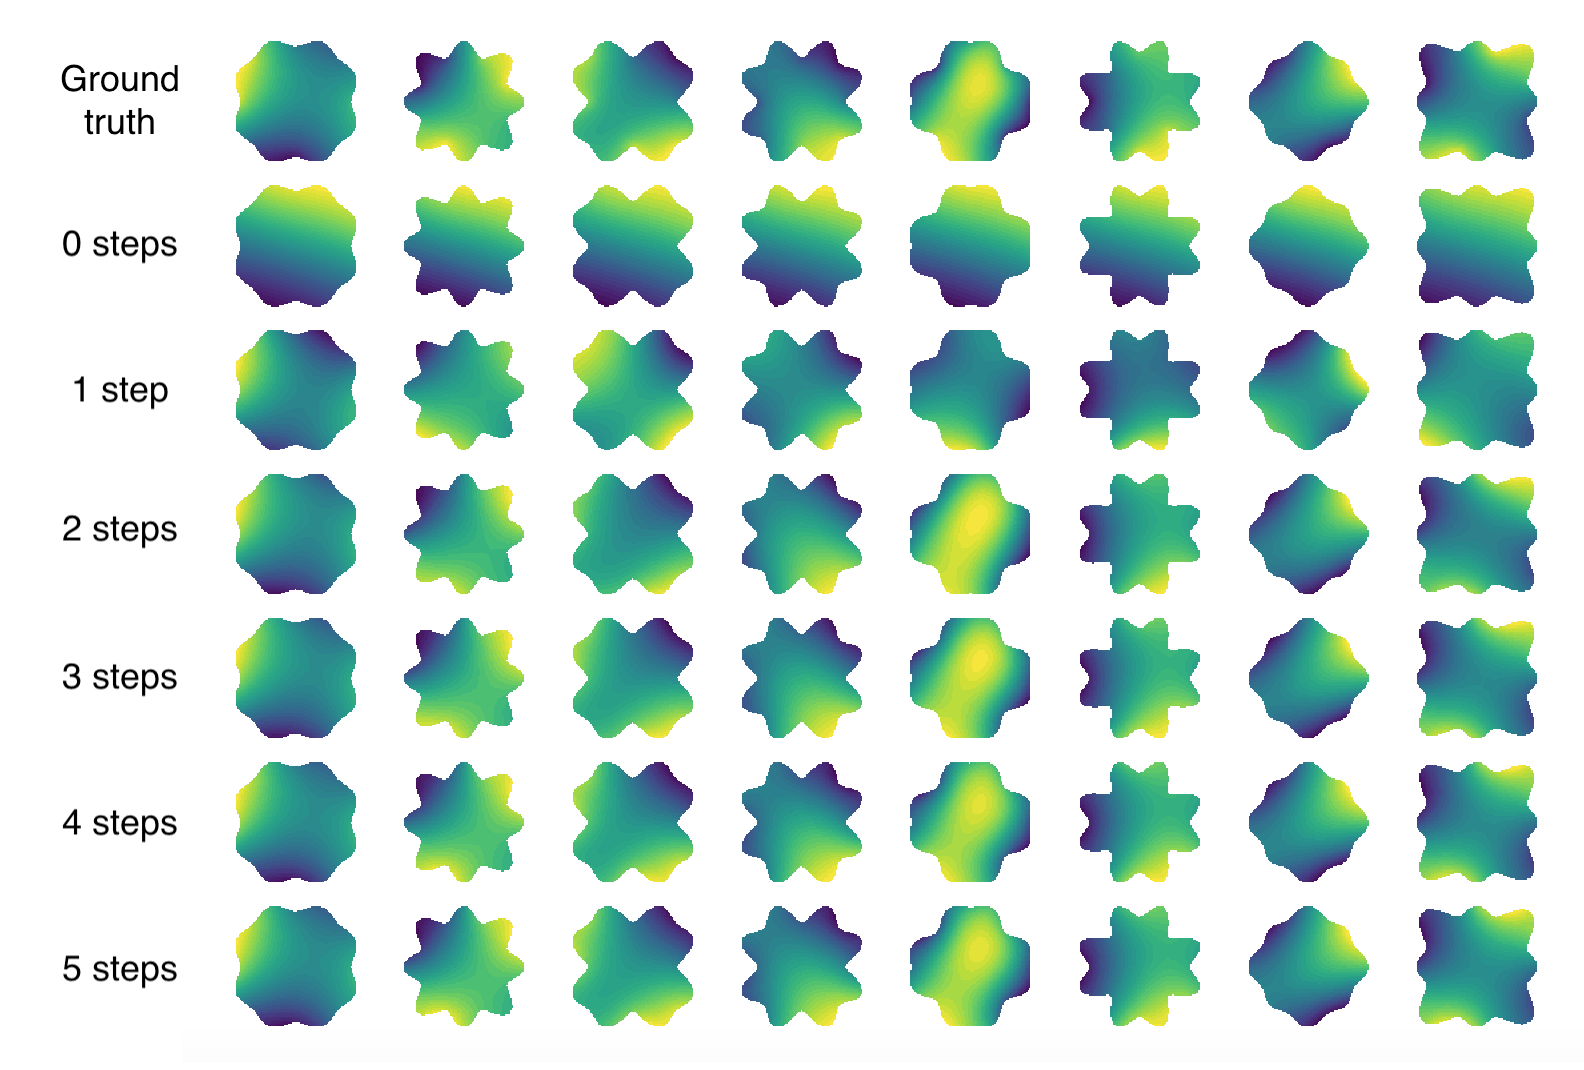
\includegraphics[width=10cm]{meta-pde/figures/poisson_meta_labeled.png}
\caption{\small
Solutions to nonlinear Poisson equations with varying domains, boundary conditions
and source terms. Top: ground truth finite element solution.
Second row: solution represented by Meta-PDE initial neural network parameters.
Third row onwards: solution after each gradient step in the Meta-PDE inner loop.}%
\label{fig:results_per_step}%
\end{figure}

Meta-PDE learns to quickly find solutions with low error. Table \ref{tbl:results}
shows the mean squared solution error and solution time after zero through five gradient steps for
a Meta-PDE model trained to minimize the energy estimate after five gradient steps,
as compared to finite element models of varying fidelities.
The highest-fidelity finite element model was taken as ground truth and was used to
compute errors.
Errors and solution times were evaluated using sixteen held-out problems from the same
distribution which were not used during training
Mean-squared errors are computed
between the value of a given approximate solution and the value of the ground truth
(highest fidelity finite element solution) at 1024 randomly sampled points within
the domain.
The relative mean-squared error is computed by dividing the mean-squared error by
the sum of squares of solution values for the ground-truth solution.
% Figure \todo{make} shows the ground truth and finite element approximations of
various fidelities for sampled test problems.
Figure \ref{fig:results_per_step} shows the ground truth and the Meta-PDE solution after
zero through five gradient steps minimizing the variational energy for
sampled test problems.


We see that Meta-PDE learns to output accurate solutions, and when run on the same
CPU (a 2.5GHz Intel i7) is about 4-7x faster than a finite element method with similar
accuracy, and about 50x more accurate than a finite element method
with the same computation cost.
Unlike finite element models, Meta-PDE can be easily accelerated by a GPU,
and on GPU we see close to 50x speed up in deployment,
leading to a 400x speed increase over similar accuracy finite element models.
We expect these gains would only increase if we replaced the vanilla fully-connected
neural network with a more tailored NN (such as the attention-like model used
to fit PDE solutions in \citet{wang2020understanding}),
used a lower-variance sampling strategy,
or more carefully tailored a meta-learning algorithm to this problem.
The speed-accuracy tradeoff could also be tuned by changing the size of the NN used
or the number of steps in the inner loop optimization.
